\documentclass[8pt, hyperref={colorlinks=true}]{beamer}
\usepackage[utf8]{inputenc}

\usetheme{CambridgeUS}

\usepackage{array}
\usepackage{makecell}
\usepackage{amsmath}
\usepackage{multirow}
\usepackage{mathtools}
\usepackage{graphicx}

\newcommand{\team}{IMMC Team \#18859084\hphantom{a}}

\usepackage[style=british]{csquotes}

\def\signed #1{{\leavevmode\unskip\nobreak\hfil\penalty50\hskip1em
  \hbox{}\nobreak\hfill #1%
  \parfillskip=0pt \finalhyphendemerits=0 \endgraf}}

\newsavebox\mybox
\newenvironment{aquote}[1]
  {\savebox\mybox{--- #1}\begin{quote}}
  {\vspace*{1mm}\signed{\usebox\mybox}\end{quote}}

\title{Thesis Presentation IMMC 2018 International\\IMMC Team \#18859084}

% A subtitle is optional and this may be deleted
\subtitle{Quantitative Methods for the Evaluation of Hospital Performance}

\author{Liu, R.\and Shan, J.\and Zhang, T.\and Zhang, Y.}

\date{Apr. $27^{\mathrm{th}}$, 2018}

\subject{Mathematics and Applied Mathematics}

%\AtBeginSubsection[]
%{
%  \begin{frame}<beamer>{Outline}
%    \tableofcontents[currentsection,currentsubsection]
%  \end{frame}
%}

\begin{document}

\begin{frame}
  \titlepage\footnote{Team members' names are sorted in ascending lexicographical order.}
  \begin{aquote}{Hippocrates of Kos}
      Wherever the art of medicine is loved, there is also a love of humanity.    
      \end{aquote}
\end{frame}

% \begin{frame}{Outline}
%   \tableofcontents
%   % You might wish to add the option [pausesections]
% \end{frame}

% Section and subsections will appear in the presentation overview
% and table of contents.
\section{Introduction}

\subsection{Problem Restatement}

% \begin{frame}{Background}

%   In the IMMC 2018 International Round, Team IMMC \#18859084 proposed a prototypical method to evaluate the performance of medical institutions\footnote{henceforth and in the thesis referred to interchangeably as "hospitals"} and assist producing the optimal selection.\\~\
  
%   As required in the contest question, in the thesis the measure of quality of medical institutions with death rate\footnote{henceforth and in the thesis referred to interchangeably as "mortality"} and the measure with other criteria\footnote{henceforth and in the thesis referred to interchangeably as "factors"} in additional to mortality are developed.

% \end{frame}

% \begin{frame}{Methodology}
%   In the thesis, the performance of medical institutions is evaluated with following criteria:
%   \begin{itemize}
%   \item{
%     Mortality
%     \begin{itemize}
%         \item General Mortality
%         \item Distribution of Mortality over Patients' Age
%         \item Distribution of Mortality over Patients' Biological Sex
%     \end{itemize}
%   }
%   \item{
%     Treatments
%     \begin{itemize}
%         \item Accuracy of Diagnoses
%         \item Effectiveness of Treatments
%     \end{itemize}
%   }
%   \item{
%     Services
%     \begin{itemize}
%         \item Service Quality
%         \item Waiting and Queuing
%     \end{itemize}
%   }
%   \item{
%     Availability
%     \begin{itemize}
%         \item Institutions' Availability
%         \item Expenses
%         \item Geographical Locations and Distances
%     \end{itemize}
%   }
%   \end{itemize}

% \end{frame}

\subsection{Solution Summary}

\begin{frame}{Methodology and Summary of Results}
In the thesis, the performance of medical institutions is evaluated with following criteria:
  \begin{itemize}
  \item{
    Mortality
    \begin{itemize}
        \item General Mortality
        \item Distribution of Mortality over Patients' Age
        \item Distribution of Mortality over Patients' Biological Sex
    \end{itemize}
  }
  \item{
    Treatments
    \begin{itemize}
        \item Accuracy of Diagnoses
        \item Effectiveness of Treatments
    \end{itemize}
  }
  \item{
    Services
    \begin{itemize}
        \item Service Quality
        \item Waiting and Queuing
    \end{itemize}
  }
  \item{
    Availability
    \begin{itemize}
        \item Institutions' Availability
        \item Expenses
        \item Geographical Locations and Distances
    \end{itemize}
  }
  \end{itemize}\\~\
  
The discussion of performance and the evaluation thereof is indexed by medical institutions and categorized by departments, and for each performance item a real \textbf{quality ranking}, $Q1_{ij},Q2_{ij},\dots,Qn_{ij}\in[0,100]$, where $i$ indexes the institutions ($k$ items in total), $j$ the departments ($c$ items in total), and $Q1,\dots,Qn$ the criteria, is derived and standardized with an evaluation function $V_l:\mathbb{R}\to[0,100]$. At the end of the thesis, a unified value for each medical institution is derived, with consideration of each and every factors listed above, from a formula with a series of parameters $W_i\mathbin{\hphantom{}}(i=1,2,\dots,n)$, where $n$ denotes the total factors considered, denoting the \textbf{relative importance of factors}. In the most idealistic situation, the \textbf{optimal choice} with respect to all criteria will be the one $i_0$ with $\displaystyle{R_{i_0}=\max_{i=1,2,\dots,k}R_i}$.
\end{frame}

\section{Mortality}

\subsection{General Morality}

\begin{frame}{Mortality Measure and Applicability}
\hypertarget{frm:mortality_measure_and_applicability}{}

In order to propose an effective mortality measure, \team located a series of indicators published by the ARHQ (Agency for Research Healthcare and Quality), namely the \textbf{30-day Risk-Standardized Mortality Measure}, the \textbf{AHRQ Patient Safety Indicators} (PSIs), and the \textbf{AHRQ Inpatient Quality Indicators} (IQIs).

\begin{block}{Weighted PSI, IQI, and 30-day Risk-Standardized Mortality Measure Mortality}
\[
P_j = 100 \times \sum_{i=1}^{26} WP_i \cdot  \frac{\text{\# of deaths due to condition $i$ at hospital $j$}}{\text{\# of total discharged patients of condition $i$ at hospital $j$}}
\]
\[
I_j = 100 \times \sum_{i=1}^{32} WI_i \cdot \frac{\text{\# of inpatient deaths due to treatment $i$ at hospital } }{\text{\# of total inpatients underwent treatment }i}
\]
\[
R_j = 100 \times \sum_{i=1}^{4} WR_i \cdot \frac{\text{\# of inpatient deaths due to condition / treatment $i$ at hospital } j}{\text{\# of total hospitalized patients with condition }i}
\]
\end{block}

% \begin{definition}[30-day Risk-Standardized Mortality Measure]
%     \begin{itemize}
%             \item Acute myocardial infarction
%             \item Heart failure
%             \item Pneumonia
%             \item Unplanned re-admission rate
%         \end{itemize}
% \end{definition}

% \begin{definition}[AHRQ Patient Safety Indicators (PSIs) - Appendix A]
% A range of 26 indicators that assess the effectiveness of treatments that have immediate outcomes; best used to assess accidents
% \end{definition}

% \begin{definition}[AHRQ Inpatient Quality Indicators (IQIs) - Appendix B]
% 32 Indicators that specifically evaluate the mortality of inpatients
% \end{definition}
\end{frame}

% \begin{frame}{Mortality Measure and Weighted Ranking}

% \begin{block}{Weighted PSI, IQI, and 30-day Risk-Standardized Mortality Measure Mortality}
% \[
% P_j = 100 \times \sum_{i=1}^{26} WP_i \cdot  \frac{\text{\# of deaths due to condition $i$ at hospital $j$}}{\text{\# of total discharged patients of condition $i$ at hospital $j$}}
% \]
% \[
% I_j = 100 \times \sum_{i=1}^{32} WI_i \cdot \frac{\text{\# of inpatient deaths due to treatment $i$ at hospital } }{\text{\# of total inpatients underwent treatment }i}
% \]
% \[
% R_j = 100 \times \sum_{i=1}^{4} WR_i \cdot \frac{\text{\# of inpatient deaths due to condition / treatment $i$ at hospital } j}{\text{\# of total hospitalized patients with condition }i}
% \]
% \end{block}


% \end{frame}

\subsection{Distribution of Mortality over Patients' Age}

% \begin{frame}{Mortality Inclination on Age}
% Measures discussed previously do not take age into account, and thus the ranking may not be indicative for all patients, since some conditions and their treatments are more prevalent in certain ages, and patients generally prefer hospitals that are most effective at treating conditions that are common in their age groups.\\~\

% The component weight distribution for
% each of the three measures defined in Frame \hyperlink{frm:mortality_measure_and_applicability}{Mortality Measure and Applicability} need to vary depending on age. In other words, the component weights will actually
% be functions of age range.\\~\

% For simplicity, without loss of generality, we assume that
% \begin{block}{Assumption}
% \hypertarget{asp:age_0_100}{}
% A(5): The age of patients is between 0 to 100.
% \end{block}

% \end{frame}

\begin{frame}{Age-Adjusted Weights}
For simplicity, without loss of generality, we assume that
\begin{block}{Assumption}
\hypertarget{asp:age_0_100}{}
A(5): The age of patients is between 0 to 100.
\end{block}

\begin{definition}[Age-Adjusted Weights]
With \hyperlink{asp:age_0_100}{A(5)}, assume a finite sequence of $n$ probability density functions ${f_i(a)}:\mathbb{R}\to[0,1]$ over age, denoting the likelihood of patients of that age to seek treatment i, indexed by components to be considered $i$, is given, the \textbf{age-adjusted weights} would be a function
\[
\overline{W}_c(m,M)=\frac{\displaystyle W_c\int_m^M \! f_c\left(a\right)\, \mathrm{d}a}{\displaystyle\sum_{i=1}^{n}\left(W_i\int_m^M \! f_i\left(a\right)\, \mathrm{d}a\right)}
\]
where $c$ denotes the specific component just like before (such as one out of 26 PSI items), $n$ the total amount of components, and $m, M$ the age range ($0\leq m<M\leq 100$).
\end{definition}

An important property of the age-adjusted weights must be ensure in order to carry on the previous discussions: when every component has the same probability distribution over age, the age-adjusted weight must be consistent with the age-unadjusted weight. The proof of this, by putting $f_i(a)=f(a)$ for all $i$, would be rather simple and thus omitted.
\end{frame}

% \begin{frame}{Intuition of Age-Adjusted Weights}
% An important property of the age-adjusted weights must be ensure in order to carry on the previous discussions: when every component has the same probability distribution over age, the age-adjusted weight must be consistent with the age-unadjusted weight.
% \begin{block}{Proof of the Consistency of Age-Adjusted Weights}
% Since $W_i$ are weight multipliers,
% \[
% \sum_{i=1}^{n}W_i=1
% \]
% is a tautology, and thus
% \[
% \overline{W}_c(m,M)=\frac{\displaystyle W_c\int_m^M \! f\left(a\right)\, \mathrm{d}a}{\displaystyle\sum_{i=1}^{n}\left(W_i\int_m^M \! f\left(a\right)\, \mathrm{d}a\right)}=\frac{\displaystyle W_c\int_m^M \! f\left(a\right)\, \mathrm{d}a}{\displaystyle\int_m^M \! f\left(a\right)\, \mathrm{d}a\cdot\left(\sum_{i=1}^{n}W_i\right)}=\frac{W_c}{\displaystyle\sum_{i=1}^{n}W_i}=W_c,
% \]
% quod erat demonstrandum.
% \end{block}
% \end{frame}

\begin{frame}{Example: Hip-Replacement and Beta Distribution}
While hip replacements are generally more applicable to all skeletally mature patients, it is more frequently carried out on patients aged 60 - 80. Therefore, it seems reasonable that having low death rates for accidents in hip replacement as an IQI is valued more to older patients than younger ones. For hip replacement, the distribution of treatment over age is negatively skewed. One of the probability distributions that adhere to this property is the beta distribution $\mathrm{Beta}(\alpha,\beta)$, defined with

\begin{columns}

\column{0.475\textwidth}
\begin{definition}[Beta Distribution]
\[
\text{Beta}(\alpha,\beta)=\frac{x^{\alpha-1}(1-x)^{\beta-1}}{B(\alpha,\beta)}
\]
where
\[
B(\alpha,\beta) = \frac{\Gamma(\alpha)\Gamma(\beta)}{\Gamma(\alpha + \beta)}
\]
\end{definition}

\column{0.475\textwidth}
\begin{example}
\begin{figure}
    \centering
    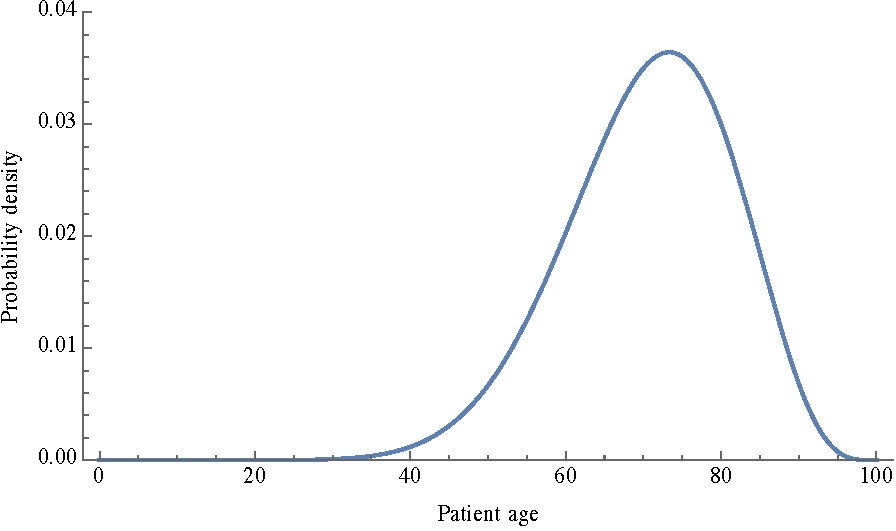
\includegraphics[scale=0.3]{hip_replacement.pdf}
    \caption{Conceptual variation of hip replacement surgeries and age}
    \label{fig:hip_replacement}
\end{figure}
\end{example}
\end{columns}
\end{frame}

% \begin{frame}{Example: Hip-Replacement and Beta Distribution}
% \begin{figure}
%     \centering
%     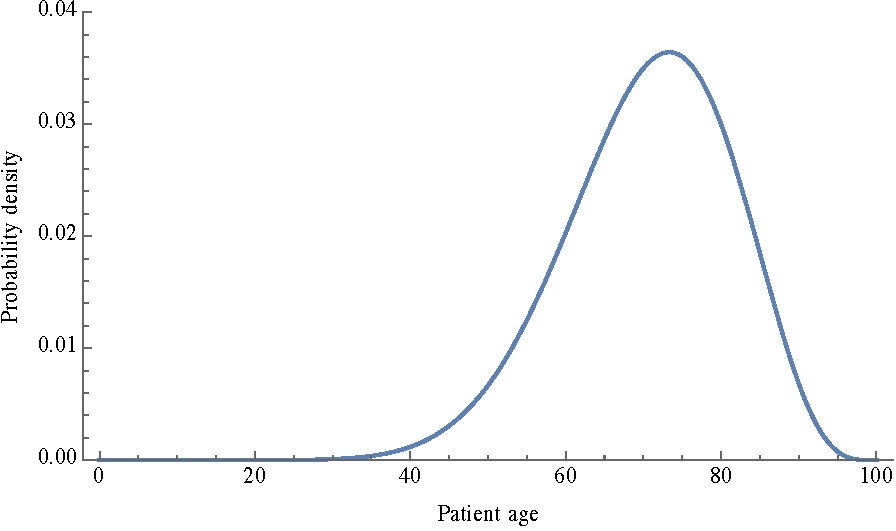
\includegraphics[scale=0.7]{hip_replacement.pdf}
%     \caption{Conceptual variation of hip replacement surgeries and age}
%     \label{fig:hip_replacement}
% \end{figure}
% \end{frame}

\subsection{Distribution of Mortality over Patients' Biological Sex}

\begin{frame}{Discrete Probability Distribution of Biological Sex}
\begin{definition}[Bio-Sex-Adjusted Weights]
Assume a finite sequence of $n$ discrete probability distribution functions $g_i(a): \{0,1\}\to[0,100]$ indexed by component indicators is given, the \textbf{bio-sex-adjusted age-adjusted weights} would be a function
\[
\overline{\overline{W}}_c\left(m, M, \phi\right) = \frac{\displaystyle g_c \left(\phi\right) \cdot \overline{W}_c\int_m^M \! f_c\left(a\right)\mathrm{d}a}{\displaystyle\sum_{i=1}^{n}\left(g_i\left(\phi\right) \cdot \overline{W}_i \int_m^M \! f_i\left(a\right) \mathrm{d}a \right)}.
\]
where $c$ denotes the specific component just like before (such as one out of 26 PSI items), $m, M$ the age range ($0\leq m<M\leq 100$), and $\phi$ the biological sex (0 for male and 1 for female, for example).
\end{definition}

The proof of the consistency of the bio-sex-adjusted age-adjusted weights is trivial and similar to the one of age-adjusted weights and thus omitted. $P_j, I_j, R_j$ can still be calculated in the similar way with $\overline{\overline{W}}_i$.
\end{frame}

\section{Treatments}

\subsection{Accuracy of Diagnoses}

% \begin{frame}{Diagnoses Outcomes}
% For a specific condition and its diagnosis, the role of the medical institution and medical professionals resembles that of a binary classifier: to determine between positive diagnosis and negative diagnosis. Thus we employ a statistics method, \textbf{Receiver Operating Characteristic (ROC) curve analysis}, to evaluate the accuracy of the diagnoses produced by a specific medical institution.

% \begin{definition}[Diagnoses Outcome]
% \centering
% \begin{tabular}{l|l|l}
%         \multirow{ 2}{*}{Result of Diagnosis} & \multicolumn{2}{c}{Actual Patient's Condition} \\
%         \cline{2-3}
%         & Positive & Negative \\
%         \hline
%         Positive & True Positive & False Positive \\
%         \hline
%         Negative & False Negative & True Negative \\
% \end{tabular}
% \end{definition}
% \end{frame}

\begin{frame}{Diagnoses Accuracy and Receiver Operating Characteristic (ROC) Curve}
\begin{definition}[Diagnoses Outcome]
\centering
\begin{tabular}{l|l|l}
        \multirow{ 2}{*}{Result of Diagnosis} & \multicolumn{2}{c}{Actual Patient's Condition} \\
        \cline{2-3}
        & Positive & Negative \\
        \hline
        Positive & True Positive & False Positive \\
        \hline
        Negative & False Negative & True Negative \\
\end{tabular}
\end{definition}

\begin{definition}[ROC Curve]
\textbf{ROC Curve} is a system of 2 parametric equations,
\[
\begin{cases}
x=\text{FPR}(t)\\
y=\text{TPR}(t)
\end{cases}
\]
where FPR and TPR are functions defined below from diagnosis threshold $t$ (for example, how sensitive should medical professionals be when identifying diseases from conditions) to \textbf{False Positive Rate} and \textbf{True Positive Rate}:
\[
\text{FPR}(t)=\frac{\text{FP}(t)}{\text{FP}(t)+\text{TN}(t)}
\]
\[
\text{TPR}(t)=\frac{\text{TP}(t)}{\text{TP}(t)+\text{FN}(t)}
\]
\end{definition}
\end{frame}

\begin{frame}{Example of ROC Curve with Demonstrative Data}
\begin{figure}
    \centering
    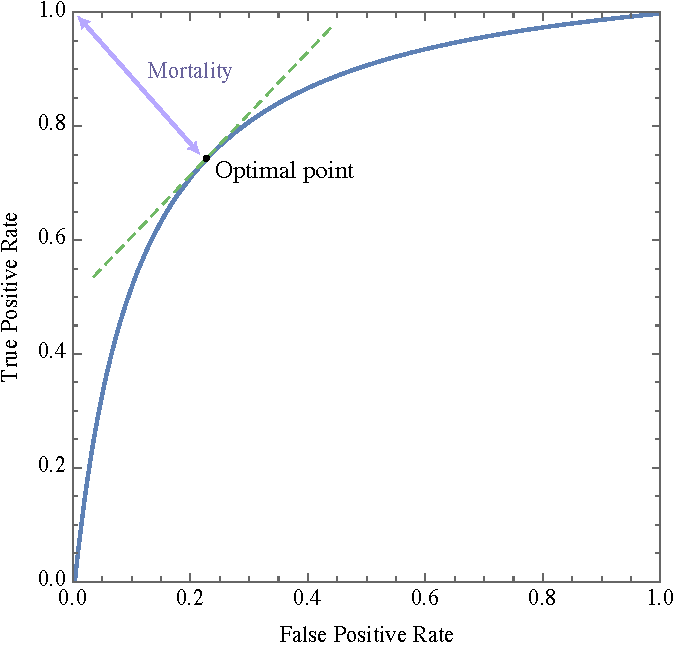
\includegraphics[scale=.58]{ROC.pdf}
    \caption{Receiver Operating Characteristic Curve for a hospital's diagnosis ability}
    \label{fig:roc}
\end{figure}
\end{frame}

\begin{frame}{Accuracy Measure}
A measure of accuracy is defined by
\begin{definition}[Accuracy of Classification]
\[
\text{ACC} = \frac{\text{TP} + \text{TN}}{\text{TP} + \text{TN} + \text{FP} + \text{FN}}
\]
\end{definition}
for a particular classifier (medical institution), changing the threshold would result in change of FPR and TPR, and this process should be continuous. In the thesis \team assumes that it is differentiable in order to proceed with the discussion of maximum accuracy.\\~\

\team did not mention an implicit assumption in the thesis, but the argument carried out implies it. We wish to make this augmentation clear now:
\begin{block}{Assumption - Augmentation}
A(13): The change of amount of people can be considered continuously differentiable up to a sufficiently high order.
\end{block}

With this assumption accepted, we will be able to dictate properties on the maximum accuracy of the classifier.
\end{frame}

\begin{frame}{Maximum Accuracy}
\begin{block}{Notational, Convention}
In the thesis, when it is defined, i.e. when it is a function from $t$ to $r(x)$, we use the notation
\[
r(x)=\text{TPR}(\text{FPR}^{-1}(x))
\]
interchangeably with the parametric equations.
\end{block}

\begin{theorem}[Location of Maximum Accuracy]
The diagnoses accuracy of a specific threshold $t_0$ is defined by the distance between the point on the ROC curve $r(x)$ of that threshold and the ideal point $(0,1)$, and the maximum accuracy of a classifier is accomplished when
\[
r'(x)=\frac{dy}{dx}=\frac{\displaystyle\frac{d\,TPR(t)}{dt}}{\displaystyle\frac{d\,FPR(t)}{dt}}=1
\]
\end{theorem}
Due to the limit of time, \team cannot draft a full-scale formal proof, thus an intuitional approach is taken.\\~\

Henceforth, the maximum accuracy of a medical institution $j$ will be denoted by $A_j$; and the ROC curve, $r_j(x)$.
\end{frame}

% \begin{frame}{Maximum Accuracy}
% \begin{proof}
% Ideally, all hospitals would want to operate at the unique point where $r'(x) = 1$. This is because the trade-off between ``lenience" and ``stringency" is kept minimum. At any $x$ where $r'(x)>1$, the hospital tends to increase its \textit{true positive rate} by being more stringent with its diagnosis, knowing that this increase comes with a relatively smaller cost (i.e.\ a less-than-proportional increase in \textit{false positive rate}). On the other hand, if a hospital is currently at a point $x$ where $r'(x) < 1$, then it should decrease its \textit{false positive rate}, knowing that it comes at a smaller cost (i.e.\ a less-than-proportional decrease in \textit{true positive rate}). Therefore, this optimal point is also where the diagnostic accuracy is maximized, and likely to be the place that the hospital operates in the long-run (due to the inverse relationship between \textit{false positive rate} and \textit{true negative rate}).
% \end{proof}
% \end{frame}

% \begin{frame}{Maximum Accuracy and Measure}
% As demonstrated in the previous figure, the maximum accuracy of a medical institution is when it reaches the point where the derivative of the parametric equations is equal to 1.\\~\

% 100 multiplied by the maximum diagnostic accuracy (in order to give a score out of 100) can then be calculated for each medical institution and used as one of the measures for mortality, assuming that both wrong treatment and lack of treatment when needed could lead to evitable deaths.\\~\

% Henceforth, the maximum accuracy of a medical institution $j$ will be denoted by $A_j$; and the ROC curve, $r_j(x)$.
% \end{frame}

\begin{frame}{Conclusion for Contest Question 1 - Mortality Measure All-in-One}
At this point, \team decides to answer contest question 1 instead of add more criteria for mortality.
\begin{block}{Contest Question 1}
Develop a model that uses mortality to measure the quality of a hospital.
\end{block}
\begin{definition}[Evaluation Function - Mortality Unified Ranking]
\begin{align*}
Q0_{ij}=V_j\left(i, P_j, I_j, A_j\right) =& 100\exp\left[\frac{(100-P_j) + (100-I_j) + A_j}{3} - 100\right] \\
& - \left(100 - \frac{(100-P_j) + (100-I_j) + A_j}{3}\right) e^{-100}
\end{align*}\footnote{At this time, the mortality measures are not department-related, so $i$ is simply a phantom parameter.}
\end{definition}
\end{frame}

\subsection{Effectiveness of Treatments}

\begin{frame}{Ranking of Success Rate of Treatments}

\begin{definition}[Evaluation Function for Success Rate]
Let $r_{ij}\in[0,100]$ denote the success rate of the department/specialty $i$ in medical institution $j$, then the ranking of success rate of treatments would be
\[
Q1_{ij}=V_{su}\left(r_{ij}\right) = 100 e^{r_{ij}-100} - (100-r_{ij})e^{-100}
\]
\end{definition}
\begin{block}{Plot with Demonstrative Parameters}
\begin{figure}
    \centering
    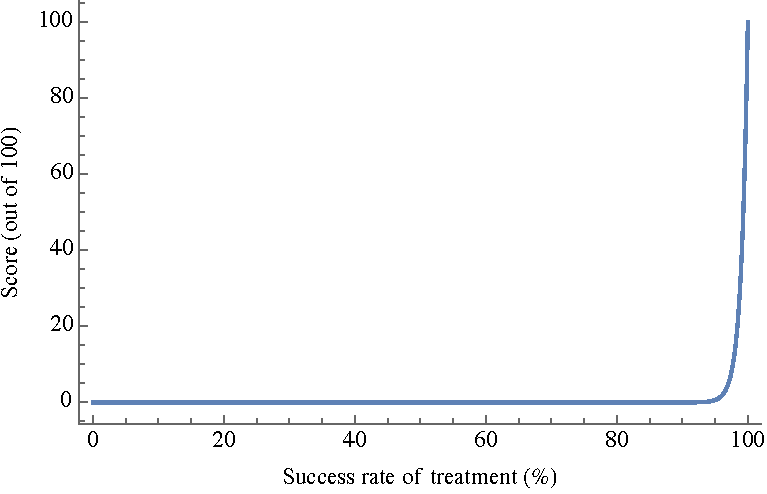
\includegraphics[scale=0.425]{success_rate.pdf}
    \caption{Relationship of success rate and success score.}
    \label{fig:success_rate}
\end{figure}
\end{block}
\end{frame}

\subsection{Performance in Controlling Epidemics}
\begin{frame}{Susceptible-Infected-Recovered Type Epidemic Disease with Medical Institution's Intervention}
\begin{block}{Alternative A}
\[
\begin{dcases}
\frac{dS}{dt}=-\frac{\beta}{N}IS-\max\{0,\min\{S,\mu\}\}\\
\frac{dI}{dt}=\frac{\beta}{N}IS-\gamma I-\max\{0,\min\{I,\nu\}\}\\
\frac{dR}{dt}=\gamma I+\max\{0,\min\{S,\mu\}\}+\max\{0,\min\{I,\nu\}\}
\end{dcases}
\]
\end{block}
\begin{block}{Alternative B}
\[
\begin{dcases}
\frac{dS}{dt}=-\frac{\beta}{N}IS-\mu S\\
\frac{dI}{dt}=\frac{\beta}{N}IS-\gamma I-\nu I\\
\frac{dR}{dt}=\gamma I+\mu S+\nu I
\end{dcases}
\]
\end{block}
\team chooses Alternative B out of 2 because it preserves more continuous properties and is easier to analyze both quantitatively and qualitatively, although Alternative A reflects the reality better.
\end{frame}

% \begin{frame}{S.I.R. Model with Medical Institution's Intervention}
% \begin{block}{S.I.R. Model with Medical Institution's Intervention}
% \[
% \begin{dcases}
% \frac{dS}{dt}=-\frac{\beta}{N}IS-\mu S\\
% \frac{dI}{dt}=\frac{\beta}{N}IS-\gamma I-\nu I\\
% \frac{dR}{dt}=\gamma I+\mu S+\nu I
% \end{dcases}
% \]
% \end{block}
% \end{frame}

% \begin{frame}{Demonstration of Medical Institution's Intervention - Non-Intervention}
% \centering
% \begin{tabular}{c|c|c}
%             Parameter & Implication & Value \\\hline
%             $\beta$ & Infection spreading efficiency & 2 \\
%             $\gamma$ & Human immune system self-curing efficiency & .1 \\
%             $N$ & Total population & 1000 \\\hline
%             $S(0)$ & Initial susceptible population & 999 \\
%             $I(0)$ & Initial infected population & 1 \\
%             $R(0)$ & Initial recovered population & 0 \\
%         \end{tabular}
% \begin{figure}
% \centering
% 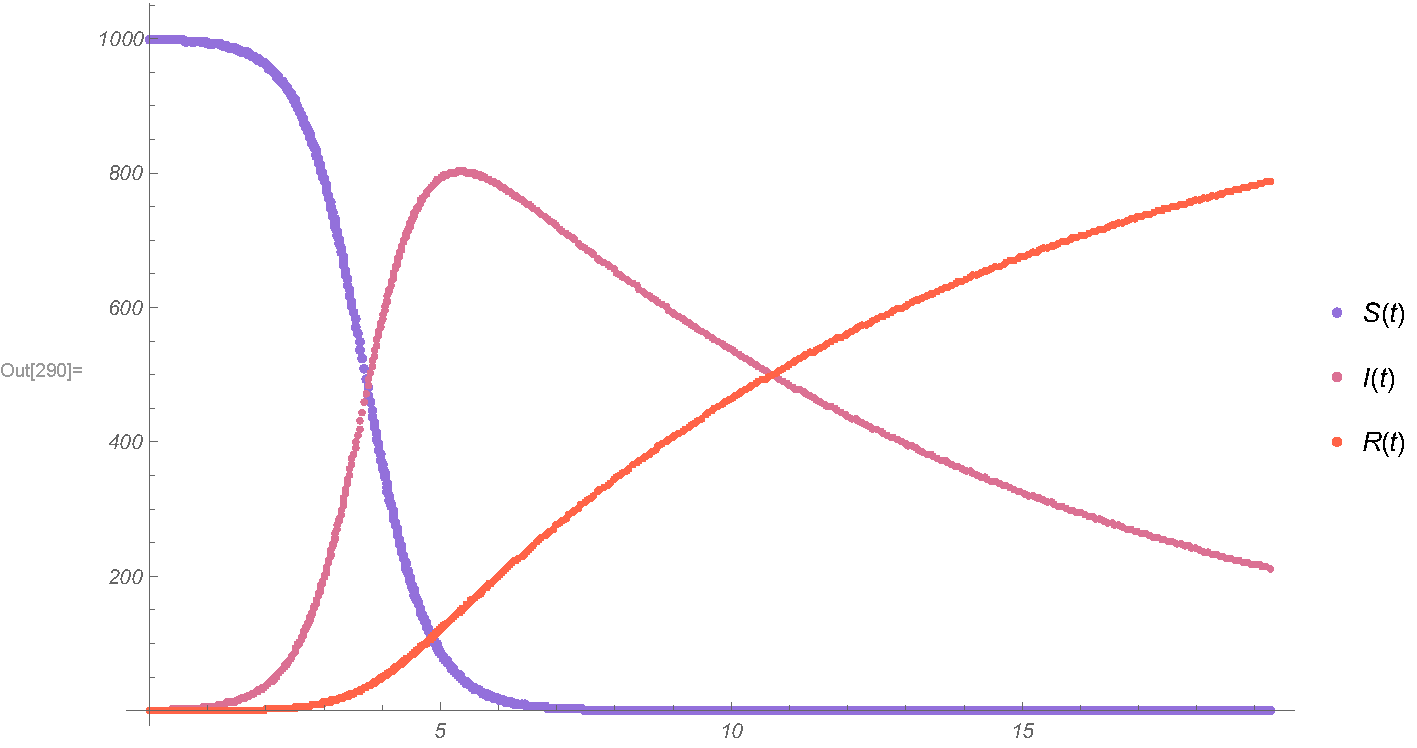
\includegraphics[scale=.4, clip, trim=37.5pt 0 0 0]{AdaptiveEulerOriginalSIR.pdf}
% \label{fig:euler_ori_sir}
% \end{figure}
% \end{frame}

% \begin{frame}{Demonstration of Medical Institution's Intervention - Intervention}
% \centering
% \begin{tabular}{c|c|c}
%          Parameter & Implication & Value \\\hline
%          $\beta$ & Infection spreading efficiency & 2 \\
%          $\gamma$ & Human immune system self-curing efficiency & .1 \\
%          $N$ & Total population & 1000 \\\hline
%          $\mu$ & Hospital's immunization program's efficiency & .1 \\
%          $\nu$ & Hospital's treatment (for infected subjects)'s efficiency & .1 \\\hline
%          $S(0)$ & Initial susceptible population & 999 \\
%          $I(0)$ & Initial infected population & 1 \\
%          $R(0)$ & Initial recovered population & 0 \\
%     \end{tabular}
% \begin{figure}
% \centering
% 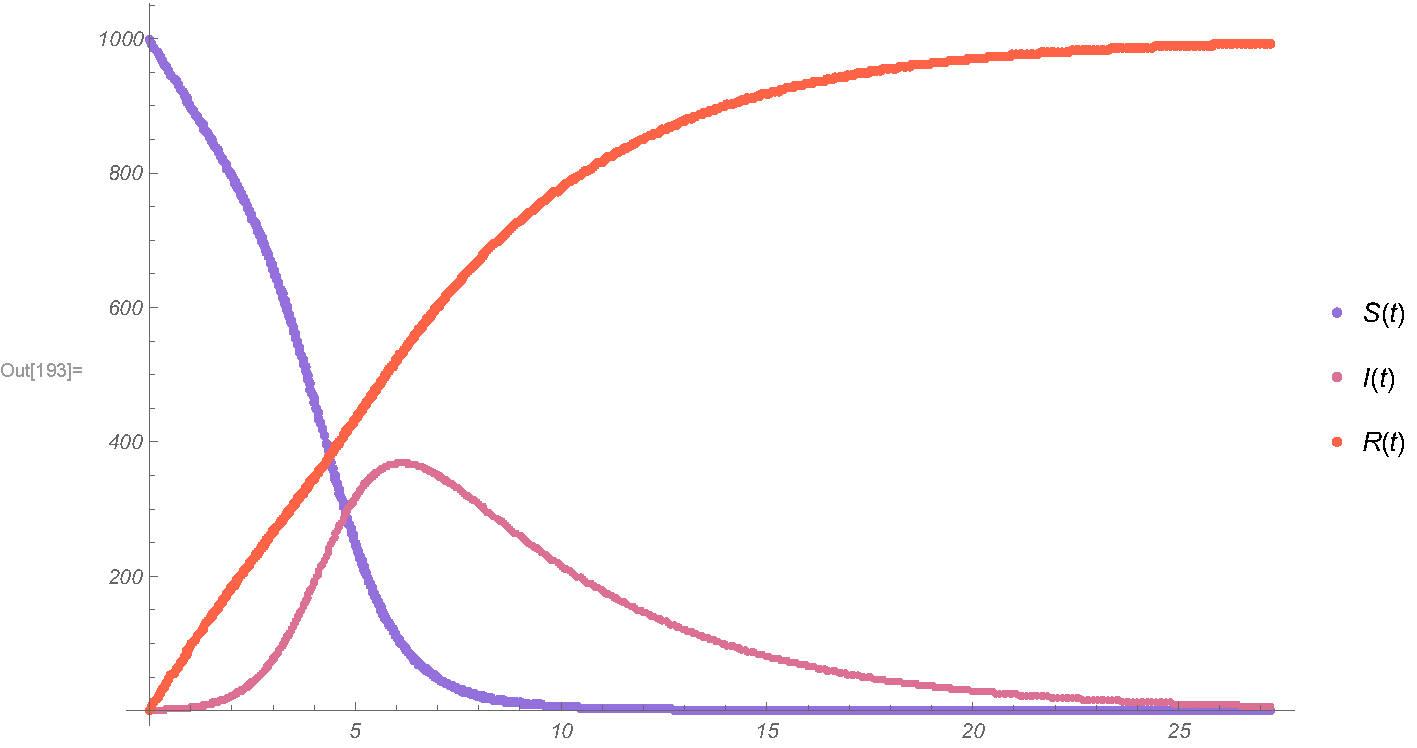
\includegraphics[scale=.375, clip, trim=37.5pt 0 0 0]{AdaptiveEulerModifiedSIR.pdf}
% \label{fig:euler_ori_sir}
% \end{figure}
% \end{frame}

\begin{frame}{Observation of Medical Institution's Intervention}
Based on the assumption that all parameters and the values of functions $S(t),I(t),R(t)$ are non-negative, we are able to conclude the monotonicity of $S(t)$ and $R(t)$ for all $t$. For the function $I(t)$, we are able to find one $t_0$ such that $I'(t_0)=0$, which is at a $t_0$ such that \[S(t_0)=\frac{N}{\beta}\left(\gamma+\frac{\nu}{I(t_0)}\right).\]

Now one might invoke the non-intervention model for comparison, where the maximum of $S(t)$ is still unique but at a $t_0$ such that \[S(t_0)=\frac{N}{\beta}r.\]\\~\

We denote the first $t_0$ as $\mathcal{T}$; the second, $T$, and $I=I(T)$ in the non-intervention one, $\mathcal{I}=I(\mathcal{T})$ in the intervention one, then the evaluation function would be defined as
\begin{definition}[Evaluation Function of Medical Institution's Intervention of Epidemics]
\resizebox{\linewidth}{!}{$\displaystyle Q4_{ij}=V_\iota\left(T_{ij},\mathcal{T}_{ij},\,I_{ij},\mathcal{I}_{ij}\right)= 100\left(1-\frac{1}{\mathrm{Re}\left(\sqrt{\mathcal{T}_{ij}-T_{ij}}\right)+1}\right)\cdot\left(\frac{\left(\sqrt{I_{ij}}+\sqrt{I_{ij}+4 \sqrt{I_{ij}}}+2\right) \mathrm{Re}\left(\sqrt{I_{ij}-\mathcal{I}_{ij}}\right)}{\left(\sqrt{I_{ij}}+\sqrt{I_{ij}+4 \sqrt{I_{ij}}}\right) \mathrm{Re}\left(\sqrt{I_{ij}-\mathcal{I}_{ij}}\right)+2 \sqrt{I_{ij}}}\right)$}
\end{definition}
\end{frame}

\begin{frame}{Demonstration of Ranking for Medical Institution's Intervention of Epidemics}
\begin{block}{Properties of Ranking Evaluation Function for Epidemics Intervention}
\centering
\begin{tabular}{c|c}
    Condition & Behaviour \\\hline
    $\mathcal{T}-T\leq0$ & $V_1=0$ \\\hline
    $\mathcal{T}-T\to+\infty$ & $V_1\to1$ \\\hline
    $I-\mathcal{I}\leq0$ & $V_2=0$ \\\hline
    $\mathcal{I}\to0$ & $V_2\to1$
\end{tabular}
\[
V=V_1\cdot V_2
\]
\end{block}

When $\displaystyle{I=\max_{t\in[0,+\infty)}I(t)=10}$, the behaviour of $V_\iota\left(T,\mathcal{T}_,\,I,\mathcal{I}\right)$ could be demonstrated with

\begin{figure}[htbp]
    \centering
    \begin{minipage}[t]{0.5\textwidth}
        \centering
        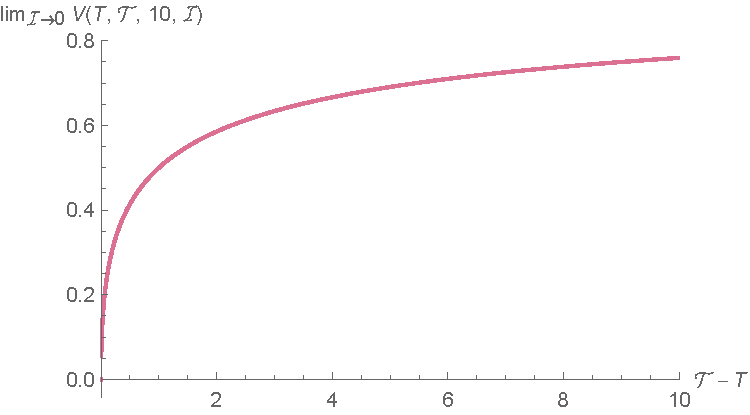
\includegraphics[width=\textwidth]{EvalFuncMSIR1.pdf} % first figure itself
    \end{minipage}\hfill
    \begin{minipage}[t]{0.5\textwidth}
        \centering
        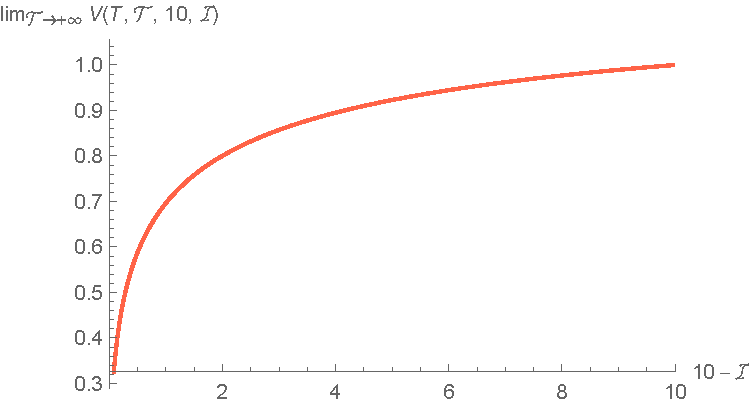
\includegraphics[width=\textwidth]{EvalFuncMSIR2.pdf} % second figure itself
    \end{minipage}
    \caption{Demonstration of 2 multipliers of the evaluation function $V_\iota\left(T,\mathcal{T}_,\,I,\mathcal{I}\right)$}
    \label{fig:msir_eval_func_plot}
\end{figure}
\end{frame}

\section{Services}

\subsection{Service Quality}

\begin{frame}{Service Quality}


\begin{definition}[Ranking for Service Quality]
\[
Q2_{ij}=V_{se}\left(p_{ij}\right) = 100e^{-_{ij}} - _{ij}e^{-100}
\]
where $p$ is the percentage of complaints from 0 to 100.
\end{definition}

This function matches the constraints $V_{se}\left(0\right) = 100$ and $V_{se}\left(100\right) = 0.$

\begin{figure}[htbp]
    \centering
    \begin{minipage}[t]{0.4\textwidth}
        \centering
        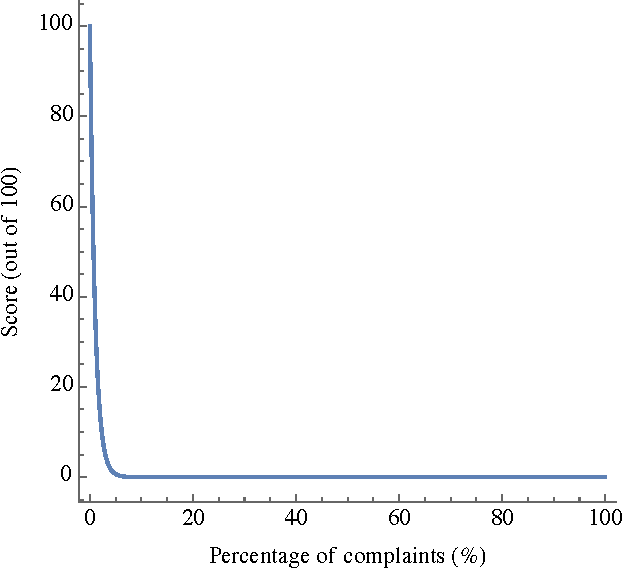
\includegraphics[scale=0.3]{service_plot.pdf}
    \end{minipage}
    \begin{minipage}[t]{0.4\textwidth}
        \centering
        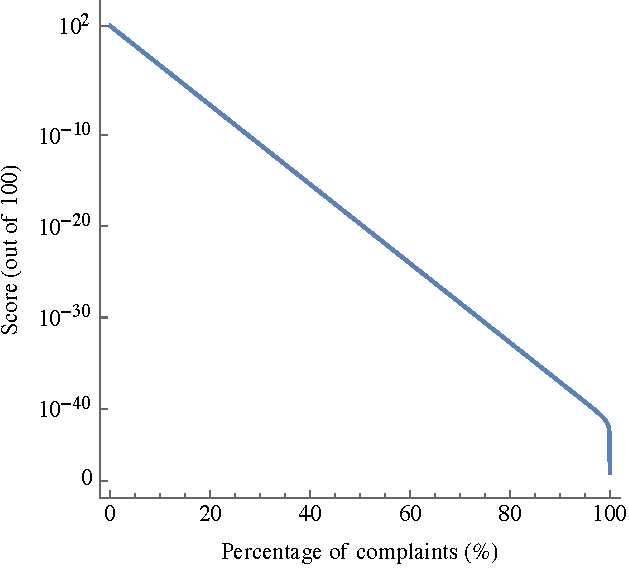
\includegraphics[scale=0.3]{log_service_plot.pdf}
    \end{minipage}
    \caption{Normal and logarithmic plot for $V_{se}\left(p_{ij}\right).$}
    \label{fig:service_plot}
\end{figure}
\end{frame}

\subsection{Waiting and Queuing}

\section{Availability}

\subsection{Waiting Time}

% \begin{frame}{Waiting Time}
% % The waiting time at a hospital can be understood as the sum of all the time they is enqueue until they leaves the hospital, or the difference between the time it takes if they enters an idle hospital and the time if they enters a fully occupied hospital. To evaluate the user experience of a hospital in terms of its availability, it requires data collected from patients in a month or year for each specialty\footnote{availability may vary across specialties}. This data can be used to curve-fit a waiting time probability density function $P_w{ij}\left(t\right)$, indexed by medical institution $j$ and department $i$, where $t$ is the total waiting time in minutes and is non-negative.\\~\

% \begin{block}{Observation}
% $$\int_0^\infty P_{ij}\left(t\right) \mathrm{d}t \le 1$$
% \end{block}
% % because this quantity represents the proportion of patients who need to wait at some point during their hospital visit, but it is possible that some patients have 0 waiting time (e.g. when the hospital is idle).\\~\

% % A common practice among hospitals in measuring patients' waiting time is by taking the median. For a continuous probability density function, the median is calculated by integrating the function from $-\infty$ and find the upper integration limit on the $x$-axis where the area equals to 0.5. However, this method is not directly applicable to $P_{ij}$ in general because it is likely that the interval $t<0$ is nonsensical. To find the median, we instead employ the \textbf{reversed median}.
% \end{frame}

\begin{frame}{Median of Waiting Time and Evaluation Function}
\begin{block}{Observation}
$$\int_0^\infty P_{ij}\left(t\right) \mathrm{d}t \le 1$$
\end{block}

\begin{definition}[Reversed Median]
The reversed median of a probability density function $P(x)$ is at $m$ such that
\[
\int_m^\infty P(x)\,\mathrm{d}x=\frac{1}{2}.
\]
If there is no such real number $m$, which implies that $\displaystyle\int_0^\infty P(x)\,\mathrm{d}x<\frac{1}{2}$, the reversed median will just be 0.
\end{definition}

\begin{definition}[Ranking of Waiting Time]
Denote $m_{ij}$ as the reversed median waiting time indexed by medical institution $j$ and department $i$, the ranking of waiting time is
\[
Q3_{ij}=V_w\left(m_{ij}\right) =
\begin{dcases}
    100e^{-m_{ij}} + \frac{m_{ij}}{20}e^{-5} & 0 < m_{ij} < 5\\
    0 & m_{ij} \ge 5 \text{ or } m_{ij} = \text{N/A}.
\end{dcases}.
\]
\end{definition}
\end{frame}

\begin{frame}{Example: Waiting Time}
Note: $m_{ij}=\text{N/A}$ iff the corresponding department of institution does not exist.\\~\

We use a set of demonstrative parameters to construct a demonstrative waiting time probability density function $P_w(t)$.
\[
P_w\left(t\right) = \frac{1.1}{1.42\pi \left[1 + \left( \frac{t -3}{1.42}\right)^2\right]}
\]

And with proper numerical method the solution of reversed median
\[
\int_m^{\infty}P_w\left(t\right) \mathrm{d}t =  \int_m^{\infty} \frac{1.1}{1.42\pi \left[1 + \left( \frac{t -3}{1.42}\right)^2\right]} = 0.5
\]
can be approximated as $m = 3.2042$, and a visualization of this would be
\begin{figure}
    \centering
    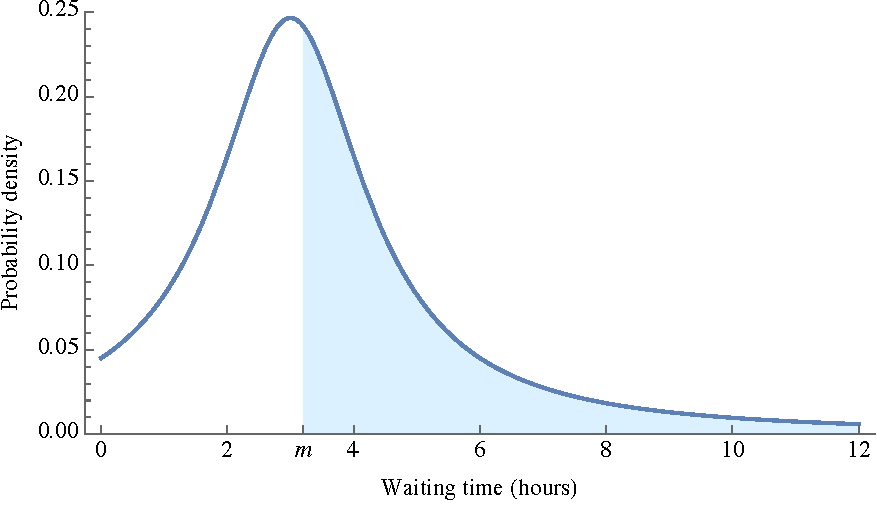
\includegraphics[scale=0.3]{waiting_time_int.pdf}
    \caption{Backward integration method to find the median waiting time for a hospital}
    \label{fig:waiting_time_int}
\end{figure}
\end{frame}

\subsection{Expenses and Geographical Distances}

\begin{frame}{Distance Distribution and Selection Bias}


\begin{definition}[Location-wise Preference Distribution]
Assume that the distance $D_i$ of every hospital $i$ to each patient is given and let $\{D_1\dots D_k\}$ be the set of distances between the patient and each of the $1\dots k$-th hospital, then the location-wise preference distribution would be
\[
P_d\left(D_i, \gamma_d\right) = \lim_{m \to 0} \frac{(D_i + m)^{-\gamma_d}}{\displaystyle\sum_{k=1}^n (D_k + m)^{-\gamma_d}}
\]
where $\gamma_d$ is the \textbf{distance selection bias}.
\end{definition}


\begin{definition}[Location-wise Preference Distribution]
Let $\{\rho_1\dots\rho_k\}$ be the price levels for each of $1\dots k$ hospitals, then the price-wise preference distribution can be defined as
\[
P_p\left(\rho_i, \gamma_p\right) = \lim_{m \to 0} \frac{(\rho_i + m)^{-\gamma_p}}{\displaystyle\sum_{k=1}^n (\rho_k + m)^{-\gamma_p}}
\]
where $\gamma_p$ is the \textbf{price selection bias}. 
\end{definition}

\end{frame}

\begin{frame}{Example: Determination of Bias}
We can determine the exact value of $\gamma_p$ by expressing it in terms of $\gamma_d$ using the result of the survey, which presents a scenario where hospital $A$ is close but expensive by 10\% of $B$ and $B$ is farther by 10\% comparing to $A$ but cheaper comparing to $A$. Since $P \left(\rho_i, \gamma_p\right)$ weighs $\beta=57\%$ and $P \left(D_i,\gamma_d \right)$ weighs $\alpha=43\%$\footnote{Appendix D}, we have

\[
\underbrace{43\% \times P_d \left(1.1,\gamma_d \right) + 57\% \times P_p \left(1, \gamma_p\right)}_{\text{P of going to the farther but cheaper institution}} = \frac{57\%}{43\%} \underbrace{\left(43\% \times P_p \left(1.1,\gamma_d \right) + 57\% \times P_d \left(1, \gamma_p\right)\right)}_{\text{probability of going to the closer but more expensive institution}}
\]

\team cites the previous work on distance bias, $\gamma_d= \log_{1.1}(2) \approx 7.2725$, and solves for
\[
\gamma_p = -\log_{1.1}\left(\frac{749}{1075 \times 328\%}\right) \approx 16.2541,
\]
which, indeed, reflects the observation that $\gamma_p > \gamma_d$.
\end{frame}

\begin{frame}{Ranking for Distances and Expanses}
\begin{definition}[Maximum and Minimum Preference Probability]
Take aside of the demonstrative parameters, with symbol $\alpha$ and $\beta$, the raw distance-price score for a medical institution $j$ would be
\[
\mu_{ij}=\alpha \cdot P\left(D_j, \gamma_d\right) + \beta \cdot P\left(\rho_j, \gamma_p\right).
\]\footnote{This ranking is independent from department index $i$.}

The minimum distance-price score $m_{ij}$ for a medical institution $j$ is defined as
\[
m_{dp}=\min_{j = 1\dots k} \left[\alpha \cdot P\left(D_j, \gamma_d\right) + \beta \cdot P\left(\rho_j, \gamma_p\right)\right].
\]

And similarly the maximum
\[
M_{dp}=\max_{j = 1\dots k} \left[\alpha \cdot P\left(D_j, \gamma_d\right) + \beta \cdot P\left(\rho_j, \gamma_p\right)\right].
\]
\end{definition}
\end{frame}

\begin{frame}{Ranking for Distances and Expanses}
Now consider $V_{dp}\left(\mu_{ji}\right)$, the evaluation function for distance and price ranking that assigns a score out of 100 for each of the hospitals purely based on their location to the patient and their pricing. The properties we wish this function to possess are
\begin{enumerate}
    \item $V_{dp}\left(\mu_{ji}\right)$ is maximized (=100) when $\mu_{ji} = M_{dp}$; and
    \item $V_{dp}\left(\mu_{ji}\right)$ is minimized (=0) when $\mu_{ji} = m_{dp}$.
\end{enumerate}

\begin{definition}[Ranking for Distance and Expanses]
\[
Q5_{ij}=V_{dp}\left(\mu_{ij}\right) = 100e^{\mu_{ij} - M_{dp}} - \frac{M_{dp} - \mu_{ij}}{M_{dp} - m_{dp}}100e^{-m_{dp}}
\]
\end{definition}

The evaluation function obviously satisfies these properties, and the visualization of the evaluation function would be

\begin{figure}[htbp]
    \centering
    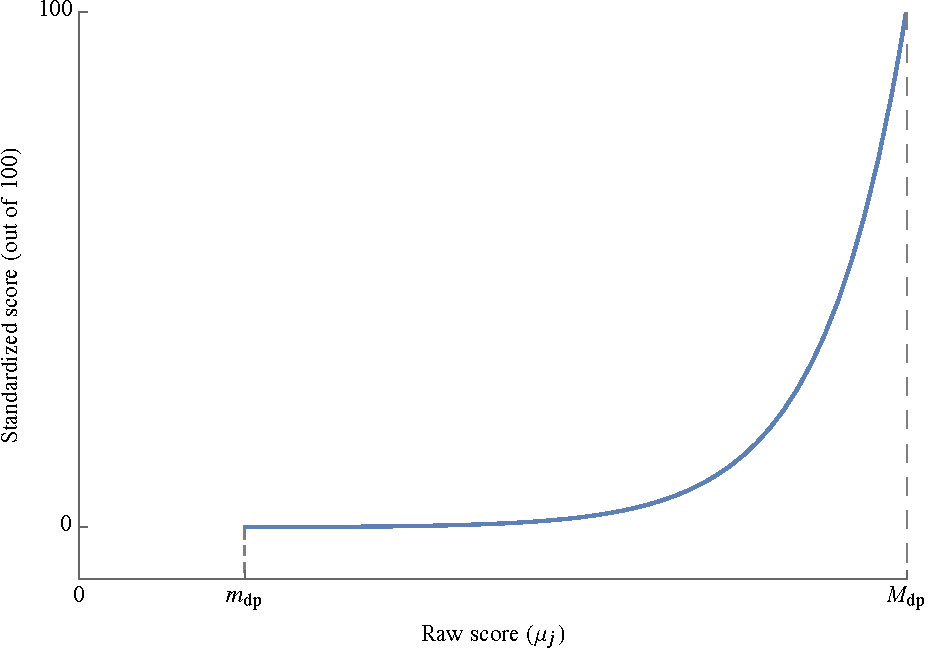
\includegraphics[scale=.3]{v_dp.pdf}
    \label{fig:v_dp}
\end{figure}
\end{frame}

\section{Conclusion}

\subsection{Relative Importance of Factors and Unified Ranking}

\begin{frame}{Quality Indicators, Unified Ranking, and Contest Question 2}

\begin{block}{Contest Question 2}
Develop a model that uses other factors, in addition to mortality, to measure the quality of a hospital. Based on the factors you include from particular hospitals, your model must result in information to make a decision of which hospital is the best.
\end{block}

\begin{columns}
 
\column{0.475\textwidth}
\begin{example}
The demonstrative data we gathered for $W_i$ are\footnote{Appendix C}
\begin{tabular}{c|c|c}
        $W_i$ & Indicator & Value  \\ \hline
        $W_1$ & Mortality & 11.3\% \\
        $W_2$ & Success rate & 19.2\% \\
        $W_3$ & Service quality & 19.1\% \\
        $W_4$ & Median waiting time & 15.9\% \\
        $W_5$ & Control of epidemics & 16.4\% \\
        $W_6$ & Location and price & 18.1\%
\end{tabular}
\end{example}

\column{0.475\textwidth}
\begin{block}{Unified Ranking}
In the thesis we submitted, a matrix-formed notation is employed for determining the unified ranking, but now for simplicity we wish to restate it as
\[
R_i=\sum_{j=1}^c\sum_{l=1}^nW_l\cdot Ql_{ij}
\]
where $i$ indexes medical institutions $1,2,\dots,k$.
\end{block}
\end{columns}

\vspace{.15cm}

And the optimal decision would be medical institution $i_0$ such that
\[
R_{i_0}=\max_{i=1,2,\dots,k}R_i.
\]

\end{frame}

% \subsection{Reflections and Future Developments}

% \begin{frame}{Reflections and Future Developments}
% \begin{itemize}
% \item Because the time and funds are limited, this time it’s only a preliminary experiment.
% \item The next research should include a large sample size, being done via WeChat, network, telephone.
% \end{itemize}

% First, we should partition the whole country and allocate the sample size according to the proportion of population in the region. The sample size should be calculated according to the specific stratified sampling, and it should be estimated to exceed 10 thousand.\\~\

% Then, collect and classify sample characteristics.\\~\

% Questions may include:
% \begin{itemize}
% \item General questions for preference of selecting hospitals
% \begin{itemize}
% \item doctor professional level
% \item hardware (equipment, wards environment, etc.)
% \item service quality
% \item waiting time
% \item price
% \item location
% \end{itemize}
% \item Personal questions
% \begin{itemize}
% \item age group (18-40, 41-65, above 66)
% \item annual income (below 30,000, 30,000-100,000, 100,000-300,000, above 300,00)
% \end{itemize}
% \end{itemize}

% Statistical Analysis
% \begin{enumerate}
% \item Calculate the proportion and weight according to the options.
% \item Subgroup can be stratified and analyzed according to the sample characteristics.
% \end{enumerate}
% \end{frame}


% % All of the following is optional and typically not needed. 
% \appendix
% \section<presentation>*{\appendixname}
% \subsection<presentation>*{Bibliography}

% \begin{frame}[allowframebreaks]
% \fontsize{7pt}{7.2}\selectfont
%   \frametitle<presentation>{Bibliography}
    
%   \begin{thebibliography}{9}
    

% \bibitem{tuberculosis}
% Global Tuberculosis Report 2016. Geneva: \textit{World Health Organization}, 2016 \url{http://www.who.int/tb/publications/global_report/en/}. 

% \bibitem{a}
% ``Hip Replacement." \textit{NHS Choices}, NHS, 10 June 2016, \url{www.nhs.uk/conditions/Hip-replacement/}. 
% \bibitem{b}
% 30-Day Risk-Standardized Mortality Measures. \textit{St. Joseph Hospital}, \url{www.stjosephhospital.com/media/file/30-Day Risk-Standardized Mortality Measures.pdf}. 
% \bibitem{c}
% ``Patient Safety Indicators." 2006-Feb-PatientSafetyIndicators.pdf, \textit{AHRQ}, Feb. 2006, \url{www.qualityindicators.ahrq.gov/Downloads/Modules/PSI/V30/2006-Feb-PatientSafetyIndicators.pdf}. 
% \bibitem{d}
% Zhu, Wen, et al. 1 Sensitivity, Specificity, Accuracy, Associated Confidence Interval and ROC Analysis with Practical SAS \textregistered  Implementations. \textit{Octagon Research Solutions}, \url{www.lexjansen.com/nesug/nesug10/hl/hl07.pdf}. 

% \bibitem{e}
% Schwartsmann1, Carlos Roberto et al. ``Correlation between Patient Age at Total Hip Replacement Surgery and Life-expectancy." Acta Ortopedica Brasileira 23.6 (2015): 323–325. PMC. Web. 18 Mar. 2018.
% \bibitem{f}
% ``Receiver Operating Characteristic." \textit{Wikipedia}, Wikimedia Foundation, 6 Mar. 2018, \url{en.wikipedia.org/wiki/Receiver\_operating\_characteristic}. 
% \bibitem{g}
% Zhu, Wen, et al. 1 Sensitivity, Specificity, Accuracy, Associated Confidence Interval and ROC Analysis with Practical SAS \textregistered Implementations. \textit{Octagon Research Solutions}, \url{www.lexjansen.com/nesug/nesug10/hl/hl07.pdf}. 
    
    
%   \beamertemplatebookbibitems
%   % Start with overview books.
 
%   \end{thebibliography}
% \end{frame}

% \begin{frame}[allowframebreaks]
%   \frametitle<presentation>{Acknowledgements}
    
%   \begin{thebibliography}{10}
        
    
%   \beamertemplatebookbibitems
%   % Start with overview books.
 
%   \end{thebibliography}
% \end{frame}

\end{document}
